\documentclass[conference]{IEEEtran}
\usepackage{cite}
\usepackage{amsmath,amssymb,amsfonts}
\usepackage{algorithmic}
\usepackage{graphicx}

\usepackage{textcomp}
\usepackage{xcolor}
\def\BibTeX{{\rm B\kern-.05em{\sc i\kern-.025em b}\kern-.08em
    T\kern-.1667em\lower.7ex\hbox{E}\kern-.125emX}}
\DeclareMathOperator*{\argmin}{\arg\!\min}

    
\begin{document}

\title{Examining Hoeffding Trees with SHAP}

\author{
	\IEEEauthorblockN{Bernhard Jaeger}
	\IEEEauthorblockA{
		\textit{University of Tübingen}\\
		Tübingen, Germany \\
		bernhard.jaeger@student.uni-tuebingen.de
	}
}

\maketitle

\begin{abstract}
Understanding the decisions made by machine learning models can be challenging due to their black box nature.
We investigate the additive feature attribution method SHAP (SHapley Additive exPlanations) that addresses this problem. 
Computing the shapley values which they are based on is in general NP-hard and can only be approximated with algorithms like Kernel SHAP.
For tree models there exists a specialized algorithm (Tree SHAP) that can compute exact SHAP values in polynomial time. 
We use the SHAP framework to investigate the relationship between Decision Trees and Hoeffding Trees. 
Theory tells us that a Hoeffding Tree should converge towards a Decision Tree when trained. 
In our experiments however we could not observe convergence. 
The reason for this remains unclear.
We also use the Tree SHAP algorithm as a ground truth to empirically examine the approximation error made by Kernel SHAP.
\end{abstract}

\begin{IEEEkeywords}
Tree SHAP, Kernel SHAP, Decision Tree, Hoeffding Tree
\end{IEEEkeywords}

\section{Introduction}

Being able to explain why a model makes a certain decision can be just as important as the models performance in areas where trust in a prediction is essential. However a lot of powerful modern algorithms like tree ensembles can be hard to interpret given their black-box nature. Multiple of the current methods that try to explain machine learning algorithms can be categorized in the class of 
additive feature attribution methods which we will introduce in section \ref{AFAM}. Surprisingly it turns out that they have a unique solution namely the SHAP values. We will discuss them in section \ref{SHAP} and present multiple algorithms and concepts related to them. Following that we will briefly introduce the tree models used in our experiments in section \ref{Trees}.\\
Additionally in this work we empirically investigated the following questions using the Tree SHAP algorithm:
\begin{itemize}
	\item How good is the approximation of SHAP values computed by Kernel SHAP?
	\item How fast do Hoeffding trees converge towards Decision Trees?
\end{itemize}
The experimental setup and results are described in section \ref{Experiments} and further information for reproducibility can be found in section \ref{Reproducibility}.
Our findings will be summarized in section \ref{Conclusion}.

\section{Additive Feature Attribution methods}
\label{AFAM}
Modern models of Machine Learning have become increasingly complex making it hard to explain their decisions.
To address this challenge we can go one layer of abstraction further and make a model of the model which we want to be simple enough to be interpretable again.
In \cite{b2} they coined the term explanation model for this approach of using an interpretable approximation of the original model.\\
When viewed trough this lens multiple of the current explanation methods can be categorized in the class of  \textbf{Additive Feature Attribution methods}. In \cite{b2} they defined this as methods having an explanation model that is a linear function of binary variables:\\

\begin{align}
	g(z') = \phi_0 + \sum_{i=1}^{M}\phi_i z_{i}'
\end{align}

Where g is the explanation model, $z' \in \{0,1\}^M, \phi \in \mathbb{R}$. \\
\textit{Local methods} like this first approximate their model $f(x)$ using \textit{simplified inputs} $x'$ where $x = h_x(x')$.\\
The objective is then to ensure $g(z') \approx f(h_x(z'))$ whenever $z' \approx x'$. \\
$\phi_i$ is then called the \textbf{effect} of feature i and summing up all effects approximates the output of the model $f(x)$ we wish to explain. Note that these \textit{explanation models} are now easily interpretable. We can for a prediction $f(x)$ given input $x$  say what influence or effect each component $x_i$ had on the final decision.\\
Methods falling in the category of Additive Feature Attribution methods include LIME \cite{b4}, DeepLIFT\cite{b5}, layer-wise relevance propagation \cite{b6}, Quantitive Input Influence \cite{b7}, Shapley sampling values \cite{b8} and SHAP \cite{b2}.\\

Additive Feature Attribution methods can have 3 desirable theoretical properties \cite{b2}:\\

\textbf{Local Accuracy}: \\
\begin{align}
f(x) = g(x') \text{ when } x = h_x(x') \text{ and } \phi_0 = f(h_x(0))
\end{align}
The intuition being that the explanation models output should match the original model for the simplified input (notice $x' = z'$ here). \\

\textbf{Missingness}: \\
\begin{align}
x'_i = 0 \rightarrow \phi_i = 0
\end{align}
The intuition is that feature missing in the original input may have no impact even if they are present in the simplified version. (Notice that even if $x' = 0$, $z'$ does not necessarily have to be 0).\\

\textbf{Consistency}: \\
Be $f_x(z') := f(h_x(z'))$, and $z' \setminus i$ mean $z'_i = 0$\\
For any two models f and f', if:
\begin{align}
f'_x(z') - f'_x(z' \setminus i) \geq f_x(z') - f_x(z' \setminus i)
\end{align}
for all inputs $z' \in \{0,1\}^M$. \\
Meaning that if the model changes in a way that some simplified input's contribution becomes larger.\\
Then: $ \phi_i(f', x) \geq \phi_i(f,x)$ \\
Meaning that it's inputs attribution should not become smaller.\\

Now it turns out that the only possible features for an additive feature attribution method that satisfies all 3 properties are the Shapley values defined as:\\
\begin{align}\label{ShapleyEquation}
\phi_i(f, x) = \sum_{z' \subseteq x'} \frac{|z'|!(M - |z'| - 1)!}{M!}[f_x(z') - f_x(z' \setminus i)]
\end{align}
$z' \subseteq x'$ are all $z'$ vectors where the non-zero entries are a subset of the non-zero entries in $x'$.\\
$|z'|$ represents the number of non-zero entries in $z'$.\\

This means that at least in theory additive feature attribution methods using Shapley values as effects are to be preferred over other methods. 
Unfortunately computing the exact Shapely values is in general NP-hard. \cite{b20}\\
In the next section we will introduce the SHAP framework which tries to unify these measures of feature importance and algorithms that try to deal with this problem.

\section{SHAP values}
\label{SHAP}
SHAP (SHapley Additive exPlanations) values \cite{b2} are obtained by solving equation \ref{ShapleyEquation} using a conditional expectation function of the original model:
\begin{align}
f(h_x(z')) = E[f(z) | z_S]
\end{align}
S is the set of non-zero indexes in $z'$. 
The mapping function is therefore implicitly defined as:\\
\begin{align}
h_x(z') = z_S
\end{align}
$z_S$ has missing values for features not in the set S.\\
Since models can not in general handle missing inputs $f(z_S)$ is approximated with $E[f(z)| z_S]$ in SHAP.\\
The intuition being that SHAP values  calculate the attribution (or effect) of each feature using the change in expectation of the model prediction when you condition on that feature. 
The feature $\phi_0 = E[f(z)]$ is the base value or the prediction the model would make if it had no observation. 
The following $\phi_i$ are then calculated by conditioning on some input features and averaging over all possible orderings of them.
As mentioned already earlier the exact computation of SHAP values can be challenging. 
Assuming feature independence (equation \ref{independence}) and model linearity (equation \ref{linearity}) one can make the computation much easier. 
\begin{align}
f(h_x(z')) &= E[f(z)|z_{S}]\\
&= E_{z_{\overline{S}}|z_S}[f(z)]\\
&\approx E_{z_{\overline{S}}}[f(z)] \label{independence}\\ 
&\approx f([z_S, E[z_{\overline{S}}]])  \label{linearity}
\end{align}
These are strong assumptions as a lot of models are non-linear and features are in general not independent of each other (e.g. a pixel value only has a meaningful interpretation when put into the context of the surrounding pixels).\\
In the following subsections we will discuss algorithms for computing or approximating SHAP values.

\subsection{Kernel SHAP (Linear Lime + Shapely Value)}
Kernel SHAP \cite{b2} is the only method presented here that can be applied to any model.
It is based on linear Lime which is a method that minimizes the following objective function:
\begin{align}
\xi = \argmin_{g \in G} L(f,g,\pi_{x'}) + \Omega(g) \label{Lime}
\end{align}
Where L is a loss function, omega a regularisation term and $\pi_{x'}$ a local kernel weighting the simplified inputs.
Lime is a linear explanation model that locally approximates the model around a given prediction.
Kernel SHAP now chooses $\Omega, \pi$ and $L$ in a way that recovers the Shapely Values (and therefore guarantees the properties missingness, local accuracy and consistency). This is possible because LIME is a additive feature attribution method. It lead to the following equations:
\begin{align}
\Omega(g) &= 0\\
\pi_{x'}(z') &= \frac{(M - 1)}{(M \text{ } choose \text{ } |z'|)|z'|(M - |z'|)}\\
L(f,g,\pi_{x'}) &= \sum_{z' \in Z}[f(h_x(z')) - g(z')]^2 \pi_{x'}(z')
\end{align}
Because the loss is quadratic and $g(z')$ is assumed to be linear we can solve equation \ref{Lime} using linear regression (and calculate the shapely values using weighted linear regression). 
The simplified input mapping $h_x(z')$ used by LIME is equivalent to equation \ref{linearity} and we can therefore use Kernel SHAP to estimate the SHAP values on every model.\\
To summarize Kernel SHAP is a model agnostic algorithm that under the assumptions model linearity and feature independence approximates the SHAP values. The time complexity of the algorithm is exponential in the number of input features M : $O(M2^M)$\cite{b2}.\\
An additional problem that arises in practice is that most models can not handle arbitrary patterns of missing inputs at inference time (which is a requirement to compute the Shapley values).
Implementation of the algorithm therefore make further approximations by replacing missing features with random values from a background dataset provided by the user (e.g. the training set). 
%TODO recheck statement
Given these limitations one can question whether the explanations provided by Kernel SHAP can be trusted in a realistic setting.\\
Better algorithms for calculating SHAP values for specific model types exist. 
Some of which will be covered in the following subsections:\\

\subsection{Linear SHAP}
For a linear model $f(x) = \sum_{j=1}^M w_j x_j + b$ you can approximate the SHAP values by only assuming feature independence (equation \ref{independence}).
The features will then be:
\begin{align}
\phi_0(f,x) = b
\phi_i(f,x) = w_j(x_j - E[x_j]) 
\end{align}
Notice that a difference to just looking at the weights is that Linear SHAP takes the difference to the baseline into account.

\subsection{Deep SHAP}
Deep SHAP \cite{b2} is an algorithm that combines shapely values with DeepLIFT \cite{b5}.
It combines SHAP values that are analytically computed for smaller components of the network and combines them into SHAP values for the whole network. Doing so we are linearising the non linear components of the network and the way in which we do this is uniquely specified by the Shapley values.
To calculate the expectation needed for SHAP we again have to assume that the input features are independent and that the deep models is linear. 
Notice that the second assumption is always violated as the point of adding depth to a neural network is that it becomes non-linear.
Further details on the algorithm are omitted here an can be found in \cite{b2}.

\subsection{Tree SHAP}
The previously discussed algorithms were all approximations of the SHAP values. The Tree SHAP \cite{b1} algorithm is able to compute \textbf{exact} SHAP values in \textbf{polynomial} time complexity for tree ensemble methods: $O(TLD^2)$. 
T here is the number of trees in the ensemble, L is the maximum number of leaves in any of the trees and D is the maximum depth of any of these trees. 
This means that the algorithm is tractable even for high dimensional data (which Kernel Shap due to the exponential time complexity is not).\\
Global feature importance of trees can also be computed with methods based on Gain \cite{b9}, Split Count \cite{b10} or Permutations \cite{b11} and locally using Sabbas \cite{b12}.
However these methods are inconsistent, meaning features can become more important while the attribution decreases. One can relate this intuitively to the definition of consistency above (but the methods here are not necessarily additive feature attribution methods hence the lack of formality).\\
Tree SHAP does not have this problem as it uses (exact) Shapely values and therefore guarantees the properties local accuracy, missingness and consistency. 
The intuition of the algorithm is that it is recursively tracking the proportion of all possible subsets flowing down into the leaves of the tree. 
Doing so the algorithm requires polynomial memory in the order $O(D^2 + M)$.
The algorithm is applicable to trees and sums of trees (which uses the fact that SHAP values of two functions added together is the sum of their individual SHAP values).\\
Note that Tree SHAP does \textbf{not} require the additional assumptions model linearity and feature independence that we had to make earlier. The algorithmic description in pseudo code can be found in \cite{b1} and an open source implementation is available at \cite{b13}.\\
The issue of missing features is addressed by approximating $f(x_S)$ using path dependent feature perturbations using the coverage information of the tree on which training samples went down which path in the tree.
This has the advantage that there is no need to provide the algorithm a background dataset.
Another variant of this algorithm uses causal interventions to exactly compute $f(x_S)$ with $E[f(X)|do(X_S = x_S)]$ \cite{b19}. 
It requires a background dataset (usually the training set) and scales linearly with the number of background samples N: $O(TLDN)$.\\
When we refer to Tree SHAP in the following we refer to the second version.\\

Now that we have a tool to precisely calculate SHAP values we can both globally for an entire dataset and locally on an individual sample inspect the importance of each feature as learned by the tree model gain insight into the model behaviour and potentially even the underlying problem if the model is good.
This analysis can even be further expanded be calculating SHAP interaction values covered next.

\subsection{SHAP interaction values}
Using the more modern Shapely interaction index \cite{b14} one can calculate interaction effects between features and store them in a matrix \cite{b1}. It's entries represent the impact of pairs of features on the model behaviour. The Shapely Interaction Index is defined as follows:\\
\begin{align}
\phi_{i,j} &= \sum_{S \subseteq N \setminus \{i, j\}} \frac{|S|!(M - |S| - 2)!}{2(M - 1)!}\nabla_{ij}(S), i\neq j \\
\nabla_{ij}(S) &= f_X(S \cup \{i,j\}) - f_X(S \cup \{i\}) - f_X(S \cup \{j\}) + f_X(S)
\end{align}

Due to it's similarity with the classical Shapely values the Shapely interaction values can be computed by using the Tree Shap algorithm twice for each feature leading to a runtime of $O(TMLD^2)$. These SHAP interaction values now allow us to distinguish between the main effect of a feature and it's interaction effect with other features. The main effect being defined as:
\begin{align}
\phi_{i,i} = \phi_i - \sum_{j \neq i} \phi_{i,j}
\end{align}


\subsection{Supervised Clustering}
Another interesting application of the individual feature attributions obtained by SHAP is called Supervised Clustering \cite{b1}. The idea is relatively straight forward. Instead of clustering features directly in an unsupervised fashion you first train an algorithm on the data using labels. You then calculate the corresponding SHAP values and then cluster on the feature attributions. With traditional clustering you have the problem that differences in the units of the features can have a large impact. With supervised clustering you don't have that problem because all attributions have the same unit as the models output. 
Fluctuations in the features value are also only considered if they are relevant for our (supervised) model.

\subsection{SHAP plots}
Now there are multiple ways to visualize the explanations generated by the SHAP framework \cite{b1}.
The most traditional would be a bar chart where the global importance of each feature is plotted as absolute value (e.g. figure \ref{fig1}). To plot the effects of a single example one can plot for example on a line how much each feature pushed the prediction of the model away from the baseline (e.g. figure \ref{fig3}).\\
Additionally you can create \textit{SHAP summary plots} which add more detail to the global view. In these features are again sorted by importance each individual attribution is then plotted as a dot plotted horizontally where the x axis show the SHAP value (effect). If multiple dots have the same SHAP value they get stacked creating an effect similar to violin plots. The actual feature value is then encoded through color.\\
\textit{SHAP dependence plots} are another visual tool where the SHAP value of a feature is plotted axis against it's feature value on the x-axis. The individual points of the test set are then displayed like a scatter plot. An additional value of a different feature can be encoded in the color of the dots.


\section{Hoeffding Trees}
\label{Trees}
Hoeffding trees \cite{b3} are a version of a Decision Tree that can be trained over time. Instead of needing all examples at once during training, they can be fed into the algorithm piece by piece for example as a stream in a database mining environment.
It's advantages are that it can be trained in constant time per example while converging towards the tree that an algorithm would learn if it had all data available at once with exponential decaying probability.\\
Decision trees, on which hoeffding trees are based, test an input at every node of the tree on an attribute and depending on the result pass it down to one of the branches of the nodes.
It finally ends up in a leaf where it is assigned a class label. 
The test at each leave is usually based on maximising some heuristic criterion like entropy or gini.
Training works by recursively replacing leaves by test nodes. 
Classic version of decision trees like CART \cite{b9} need all training examples to be available at the same time and are therefore limited by the size of the main memory.
However in order to find the best criterion to split at a given node it might already be sufficient to only look at a small amount of training samples. Deciding how many examples are needed until you make a decision can be done using a result from statistics known as the Hoeffding bound \cite{b18}.
It supposes we have made n independent observations over a real valued random variable r (of range R).
Then with probability $ 1 - \delta $ the true mean of the variable is at most $\epsilon$ away from the empirical mean:
\begin{align}
\epsilon = \sqrt{\frac{R^2 ln(\frac{1}{\delta})}{2n}}
\end{align}
The hoeffding tree algorithm now uses this bound to make the decision of how many samples to accumulate before splitting on an attribute.
It guarantees asymptotic convergence towards a batch learned tree. \cite{b3}\\
In the following sections we take a look at a hoeffding trees behaviour in an empirical fashion.

\section{Experiments}
\label{Experiments}
%TODO describe motivation of experiments

\subsection{Setup}
The dataset we used for our experiments was the UCI Adults dataset \cite{b15}. 
The objective for this dataset is to predict from demographic data if the person is going to make more than 50.000\$ a year (or not).
During preprocessing we replaced missing values ("?")  with the most frequent attribute of the respective column.
People who make less than 50k a year were labelled with 0 and the other once with 1.
Because the sklearn decision tree implementation does not support mixed type (categorical and numeric) input data we converted categorical values to numerical ones using the sklearn label encoder. 
This is likely going to lead to worse performance of the model.
However since we were not interested in building high accuracy models this should not matter.\\

As models we used the DecisionTreeClassifier from sklearn and HoeffdingTreeClassifier from scikit-multiflow.
For the split criterion we used gini for both models. 
All the other hyper-parameters did unfortunately not have an overlap between the two libraries. 
Notably we set the min\_sample\_split parameter of the decision tree to 1000 (which stopped the model from over-fitting) and the leaf\_prediction of the Hoeffding Tree to ``mc'' (because we think that it coincides best with the decision tree).\\

\subsection{Experiments}

We then trained both trees on the entire training set (consisting of 32561 data samples).
Additionally we trained another Hoeffding tree by feeding it each sample individually.
By plotting the train and test accuracy every 5000 samples we observed that the Hoeffding tree trained on individual samples converged to the Hoeffding tree trained on all data at once. 
The resulting trees both had the exact (16 digits) same training and test accuracy suggesting that the exact same tree structure has emerged.\\
Somewhat surprisingly the Decision Tree showed a difference in accuracy compared to the Hoeffding tree (in the configuration described here about 3 percent). 
Theory tells us that Hoeffding trees should converge towards decision trees given enough data.
We also tried different combinations of hyper parameters (as said before they are quite different between the two libraries) but could not find a setting with similar performance.
Notably the decision tree heavily overfitted when min\_sample\_split was set to the default value of 2 (almost 0 training error). Increasing it substantially regularized the model until the train and test performance were similar. 
The Hoeffding tree does not have this parameter and never showed overfitting behaviour.\\
We then tried to further investigate this behaviour by using the Tree SHAP algorithm to explain what the models look for.\\
Unfortunately it turned out that the current implementation of the Tree SHAP algorithm \cite{b16} is not compatible with the scikit-multiflow library (or any other library implementing Hoeffding trees).
This is not a theoretical problem (Tree SHAP works on every tree model), the existing open source libraries are simply incompatible right now.\\
We therefore used the model agnostic Kernel SHAP algorithm instead to explain the Hoeffding Tree.
Since the Kernel SHAP as discussed before is really slow we had to restrict the analysis to a background dataset of 50 samples from the training set and calculated the SHAP values for 50 samples of the test set. To stay comparable we used this subset for both algorithms.\\
Additionally for the Kernel SHAP we set the attribute l1 regularisation to ``num\_features(10)'' as suggested by the library.\\
We benchmarked the performance of both algorithms using the ipython notebook command \%\%time. Our hardware setup can be found in section \ref{Reproducibility}\\
Tree SHAP was able to calculate the SHAP values for the Decision Tree in only 15ms wall time.\\
Even with this small subset of the data Kernel SHAP still needed 4 minutes and 49 seconds wall time.
For the full test set the algorithm seemed to be intractable.\\
Using the calculated SHAP values we investigated the models overall using summary bar plots which can be seen in figure \ref{fig1} and figure \ref{fig2}. An individual prediction from the test set is visualized in figure \ref{fig3} and figure \ref{fig4}.\\

\begin{figure}[htbp]
\centerline{
	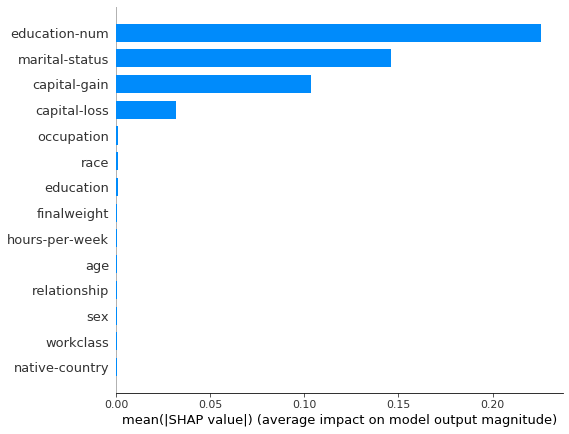
\includegraphics[width=\linewidth]{../fig/ex_01_KernelShap_HoeffdingTree_50_Samples_SummaryPlot.png}
}
\caption{Summary plot of a Hoeffding Tree explained with Kernel SHAP using 50 samples}
\label{fig1}
\end{figure}

\begin{figure}[htbp]
\centerline{
	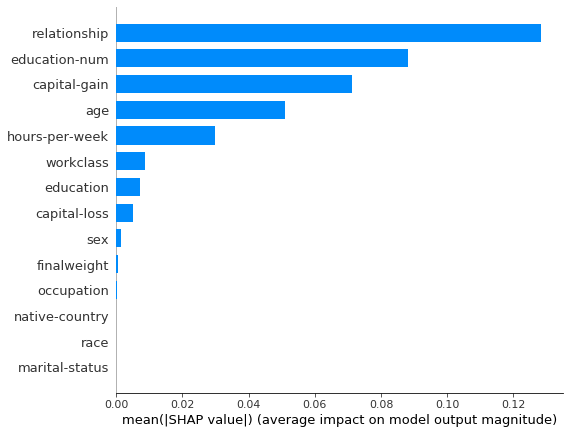
\includegraphics[width=\linewidth]{../fig/ex_01_TreeShap_DecisionTree_50_Samples_SummaryPlot.png}
}
\caption{Summary plot of a Decision Tree explained with Tree SHAP using 50 samples}
\label{fig2}
\end{figure}

\begin{figure*}[htbp]
\centerline{
	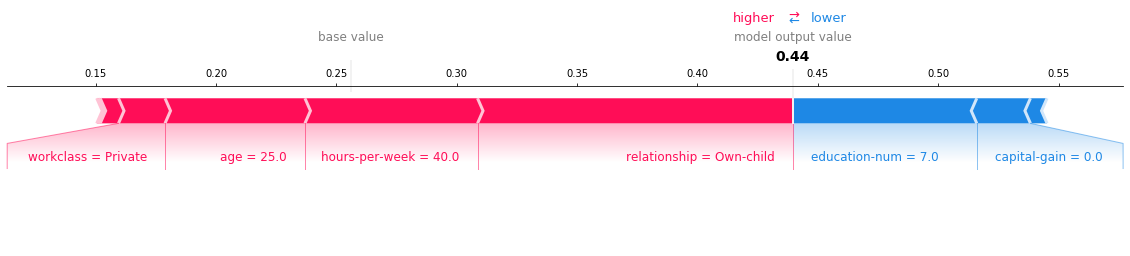
\includegraphics[width=\textwidth]{../fig/ex_01_TreeShap_DecisionTree_50_Samples_ForcePlot_sample_1.png}
}
\caption{Force plot of a Decision Tree explained with Tree SHAP using 50 samples}
\label{fig3}
\end{figure*}

\begin{figure*}[htbp]
\centerline{
	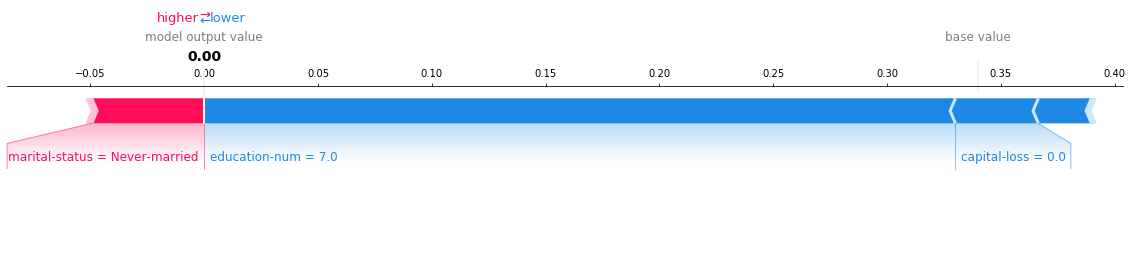
\includegraphics[width=\textwidth]{../fig/ex_01_KernelShap_HoeffdingTree_50_Samples_ForcePlot_sample_1.png}
}
\caption{Force plot of a Hoeffding Tree explained with Kernel SHAP using 50 samples}
\label{fig4}
\end{figure*}

One can clearly see that the two models look for different attributes when making their predictions and even on the attributes they agree upon (like education-num) the magnitude of their importance varies.\\
Explaining the observation that the Hoeffding tree doesn't necessarily converge to a decision tree in practice remains an open question.
Some hypothesis we have are: Differences in library implementation, Hoeffding trees assume a stationary distribution (it is unclear if this dataset is stationary), convergence guarantees are only asymptotic so the convergence could be too slow to be observed here.\\

We used the Kernel SHAP algorithm to explain the Hoeffding tree here. Since Kernel SHAP only approximates the SHAP values one natural question one might ask is how large the difference is to the exact SHAP values.
Fortunately with Tree SHAP we are now able to create a ground truth to compare the output to (at least for trees).\\
We therefore conducted a second experiment to get an empirical answer (or intuition) to this question.
We have trained a decision tree on adults just like in the last experiment. 
We now calculate the SHAP values for the decision tree both algorithms. 
Since Kernel SHAP ran faster on the decision tree we increased the number of test and background samples to 100 on both algorithms for comparison.
Additionally we used Tree SHAP to calculate the Shapely Values for the entire Test set using the entire training set as background data.
Tree SHAP on the entire test set ran in only 2.25 seconds wall time. On the 100 sub-samples it took 22.1 ms wall time and Kernel SHAP needed 1 minute 13 seconds wall time to finish it's computation.
The summary plots can be seen in figure \ref{fig5}, \ref{fig6}, \ref{fig7}.

\begin{figure}[htbp]
\centerline{
	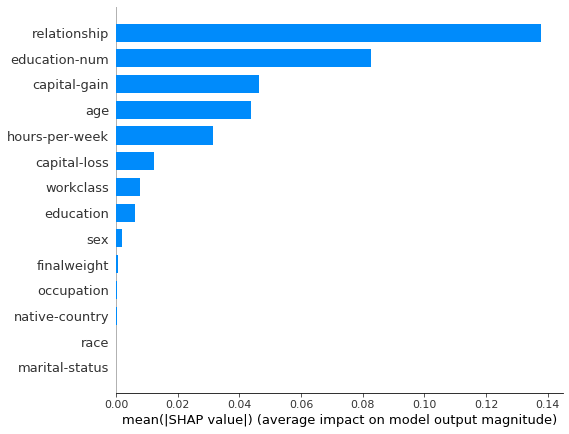
\includegraphics[width=\linewidth]{../fig/ex_02_TreeShap_16281_Samples_SummaryPlot.png}
}
\caption{Summary plot of a decision tree explained with Tree SHAP over 16281 samples}
\label{fig5}
\end{figure}

\begin{figure}[htbp]
\centerline{
	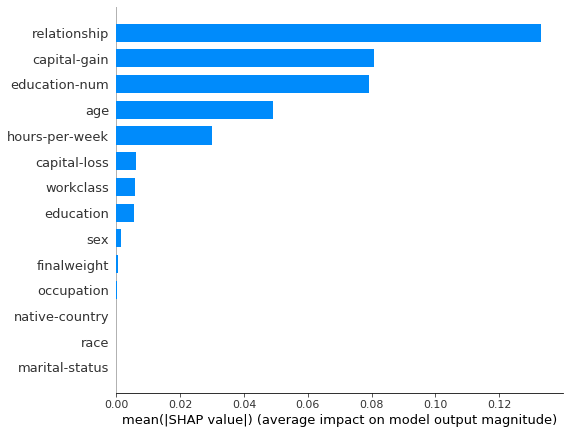
\includegraphics[width=\linewidth]{../fig/ex_02_TreeShap_100_Samples_SummaryPlot.png}
}
\caption{Summary plot of a decision tree explained with Tree SHAP over 100 samples}
\label{fig6}
\end{figure}

\begin{figure}[htbp]
\centerline{
	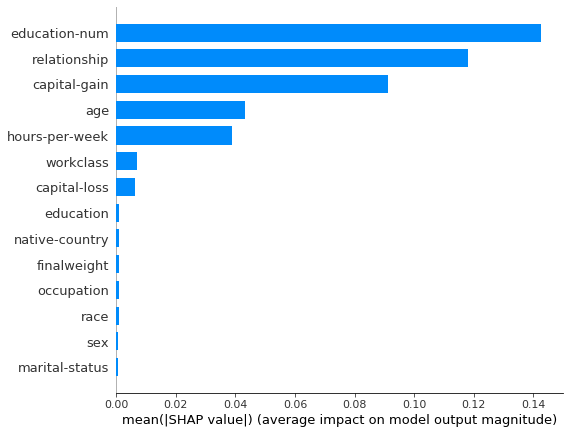
\includegraphics[width=\linewidth]{../fig/ex_02_KernelShap_100_Samples_SummaryPlot.png}
}
\caption{Summary plot of a decision tree explained with Kernel SHAP over 100 samples}
\label{fig7}
\end{figure}

Examining the summary plots one can see that through only using 100 samples we don't seem to loose a lot. Most features have similar importance and only capital-gain changed significantly.\\
Also the kernel SHAP algorithm looks like a reasonable approximation with only education-num changing significantly. 
The features that don't contribute much in the Tree SHAP plot also don't contribute much in Kernel SHAP.\\
On an individual example like shown in figures \ref{fig8} and \ref{fig9} the quantitative value of the SHAP values can be quite off even though the features that are considered stay roughly the same.\\
Observe that figure \ref{fig8} and \ref{fig3} are unsurprisingly the same because the samples used only has an impact on the average values not on the individual attributions.

\begin{figure*}[htbp]
\centerline{
	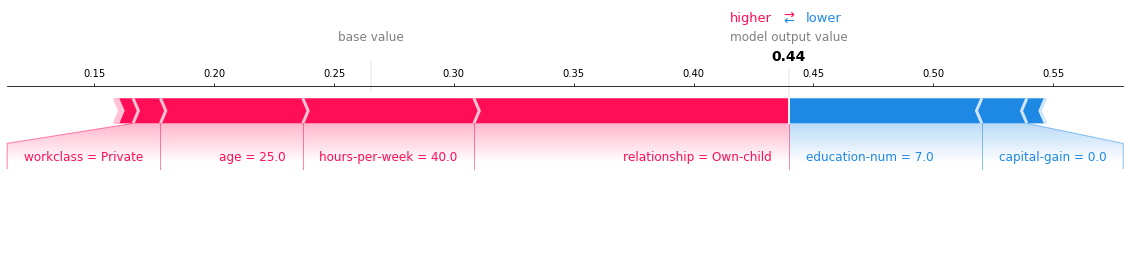
\includegraphics[width=\textwidth]{../fig/ex_02_TreeShap_100_Samples_ForcePlot_sample_1.png}
}
\caption{Force plot of a decision tree explained with Tree SHAP over 100 samples}
\label{fig8}
\end{figure*}

\begin{figure*}[htbp]
\centerline{
	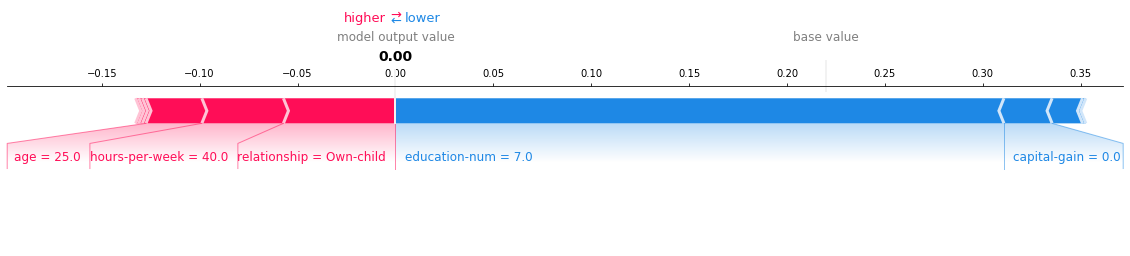
\includegraphics[width=\textwidth]{../fig/ex_02_KernelShap_100_Samples_ForcePlot_sample_1.png}
}
\caption{Force plot of a decision tree explained with Kernel SHAP over 100 samples}
\label{fig9}
\end{figure*}


\section{Conclusion}
\label{Conclusion}
We have seen that multiple current methods that aim to explain machine learning models can be categorized as additive feature attribution methods. 
These kind of methods can have three desirable properties: Local Accuracy, Missingness and Consistency.
It can be shown that the only solution to additive feature attribution methods that satisfy all 3 properties are the shapely values.
Through the SHAP framework one can approximate or compute them using algorithms like Kernel SHAP, Linear SHAP, Deep SHAP or Tree SHAP.
Using the Tree SHAP and Kernel SHAP algorithm we investigated the following questions:
\begin{itemize}
	\item Q: How good is the approximation of SHAP values computed by Kernel SHAP?\\
		  A: In our experiments we observed that the approximation of SHAP values for most feature was close to the true values. On a few features significant differences were observed.  
	\item Q: How fast do Hoeffding trees converge towards Decision Trees?\\
		  A: In our experiments we could not observe convergence. The reason for this remains an open question.
\end{itemize}

\section{Reproducibility Considerations} 
\label{Reproducibility}

In the following we list the software and hardware used for doing our experiments. 
All experiments were conducted on the same machine.
The code will be release on github at \cite{b17}.
The software library versions we used (read out using pip --freeze) are documented in table \ref{softwareVersion}.\\
 The hardware specs can be found in table \ref{hardware}.\\


%TODO this are too many remove the uneccesary once.
\begin{table}[htbp]
\caption{Software Library Versions}
\begin{center}
\begin{tabular}{|c|c|}
	\hline
	\textbf{Software library} & \textbf{Version} \\
	\hline
	Python & 3.7.4\\ \hline
	anaconda-client & 1.7.2 \\ \hline
	anaconda-navigator & 1.9.7 \\ \hline
	anaconda-project & 0.8.3\\ \hline
	conda & 4.7.12\\ \hline
	conda-build & 3.18.9\\ \hline
	conda-package-handling & 1.6.\\ \hline0
	conda-verify & 3.4.2\\ \hline
	ipykernel & 5.1.2\\ \hline
	ipython & 7.8.0\\ \hline
	ipython-genutils & 0.2.0\\ \hline
	jupyter & 1.0.0\\ \hline
	jupyter-client & 5.3.3\\ \hline
	jupyter-console & 6.0.0\\ \hline
	jupyter-core & 4.5.0\\ \hline
	jupyterlab & 1.1.4\\ \hline
	jupyterlab-server & 1.0.6\\ \hline
	matplotlib & 3.1.1\\ \hline
	notebook & 6.0.1\\ \hline
	numpy & 1.16.5\\ \hline
	pandas & 0.25.1\\ \hline
	scikit-image & 0.15.0\\ \hline
	scikit-learn & 0.21.3\\ \hline
	scikit-multiflow & 0.5.0\\ \hline                 
	scipy & 1.3.1\\ \hline
	shap & 0.35.0\\ \hline
	sklearn & 0.0\\ \hline
	
\end{tabular}
\label{softwareVersion}
\end{center}
\end{table}

\begin{table}[htbp]
\caption{Hardware Specifications:}
\begin{center}
\begin{tabular}{|c|c|}
	\hline
	\textbf{Component} & \textbf{Model} \\
	\hline
	Processor & Intel Core i7-6700 CPU\\ \hline
	RAM & 16 GB Corsair Vengeance LPX DDR4-2400\\ \hline
	GPU & NVIDIA GeForce GTX 980 \\ \hline
	Motherboard & ASUS Z170 Pro Gaming \\ \hline
	Operating system & Microsoft Windows 10 Education N \\ \hline
	Hard Drive & SSD Crucial MX200 \\ \hline
\end{tabular}
\label{hardware}
\end{center}
\end{table}


\begin{thebibliography}{00}
\bibitem{b1} Scott M. Lundberg, Gabriel G. Erion, Su-In Lee:
Consistent Individualized Feature Attribution for Tree Ensembles. CoRR abs/1802.03888 (2018).
\bibitem{b2} Scott M. Lundberg, Su-In Lee: A Unified Approach to Interpreting Model Predictions. NIPS 2017: 4765-4774.
\bibitem{b3} Pedro M. Domingos, Geoff Hulten: Mining high-speed data streams. KDD 2000: 71-80
\bibitem{b4} Marco Túlio Ribeiro, Sameer Singh, Carlos Guestrin: "Why Should I Trust You?": Explaining the Predictions of Any Classifier. KDD 2016: 1135-1144.
\bibitem{b5} Avanti Shrikumar, Peyton Greenside, Anshul Kundaje: Learning Important Features Through Propagating Activation Differences. ICML 2017: 3145-3153.
\bibitem{b6} Alexander Binder, Grégoire Montavon, Sebastian Bach, Klaus-Robert Müller, Wojciech Samek: Layer-wise Relevance Propagation for Neural Networks with Local Renormalization Layers. CoRR abs/1604.00825 (2016).
\bibitem{b7}Anupam Datta, Shayak Sen, Yair Zick: Algorithmic Transparency via Quantitative Input Influence: Theory and Experiments with Learning Systems. IEEE Symposium on Security and Privacy 2016: 598-617.
\bibitem{b8}Erik Strumbelj, Igor Kononenko: Explaining prediction models and individual predictions with feature contributions. Knowl. Inf. Syst. 41(3): 647-665 (2014).
\bibitem{b9} Leo Breiman, J. H. Friedman, R. A. Olshen, C. J. Stone: Classification and Regression Trees. Wadsworth 1984, ISBN 0-534-98053-8.
\bibitem{b10}Tianqi Chen, Carlos Guestrin: XGBoost: A Scalable Tree Boosting System. KDD 2016: 785-794.
\bibitem{b11}L Auret, C Aldrich: Empirical comparison of tree ensemble variable importance measures. Chemometrics and Intelligent Laboratory Systems, 2011 - 105, 2(2011), 157-170
\bibitem{b12}Ando Sabbas. 2014. Interpreting random forests. http://blog.datadive.net/interpreting-random-forests/ Accessed: 2020-06-15
\bibitem{b13}https://github.com/slundberg/shap Accessed: 2020-06-15
\bibitem{b14}Katsushige Fujimoto, Ivan Kojadinovic, Jean-Luc Marichal: Axiomatic characterizations of probabilistic and cardinal-probabilistic interaction indices. Games Econ. Behav. 55(1): 72-99 (2006).
\bibitem{b15}Ronny Kohavi and Barry Becker: Adult Dataset, UCI Machine Learning Repository http://archive.ics.uci.edu/ml
\bibitem{b16} https://github.com/slundberg/shap/ Accessed: 2020-07-01
\bibitem{b17} https://github.com/Kait0/EFML
\bibitem{b18} W. Hoeffding Probability inequalities for sums of bounded random variables. Journal of the American Statistical Association, 58:13-30, 1963.
\bibitem{b19} Lundberg, Scott M. and Erion, Gabriel and Chen, Hugh and DeGrave, Alex and Prutkin, Jordan M. and Nair, Bala and Katz, Ronit and Himmelfarb, Jonathan and Bansal, Nisha and Lee, Su-In, From local explanations to global understanding with explainable AI for trees, Nature Machine Intelligence 2020, volume 2, number 1 pages 2522-5839
\bibitem{b20} Yasuko Matsui, Tomomi Matsui: NP-completeness for calculating power indices of weighted majority games. Theor. Comput. Sci. 263(1-2): 305-310 (2001)


\end{thebibliography}

\end{document}
